\documentclass[border=4pt]{standalone}
\usepackage{tikz}
% Shared TikZ style: validated categorical palette (FP32 blue, FP16 orange, INT8 green, FP8 amber), light print surface.
\usetikzlibrary{arrows.meta,positioning,fit,backgrounds,calc,shapes.geometric}
\definecolor{fp32}{HTML}{2A78D6}
\definecolor{fp16}{HTML}{EB6834}
\definecolor{int8}{HTML}{1BAF7A}
\definecolor{fp8}{HTML}{EDA100}
\definecolor{ink}{HTML}{0B0B0B}
\definecolor{ink2}{HTML}{52514E}
\definecolor{muted}{HTML}{898781}
\definecolor{grid}{HTML}{E1E0D9}
\definecolor{surface}{HTML}{FCFCFB}
\definecolor{wash}{HTML}{F0EFEC}
\tikzset{
  font=\sffamily\small,
  box/.style={draw=muted, rounded corners=3pt, fill=surface, align=center, inner sep=4pt, text=ink},
  stage/.style={box, minimum height=1.0cm, text width=2.6cm},
  data/.style={box, fill=wash, draw=grid},
  result/.style={box, text width=2.9cm, minimum height=1.35cm},
  arrow/.style={-{Stealth[length=2.2mm]}, draw=ink2, line width=0.7pt},
  feedback/.style={arrow, dashed, draw=int8},
  tag/.style={font=\sffamily\scriptsize, text=ink2},
  group/.style={draw=grid, rounded corners=5pt, inner sep=6pt, line width=0.8pt},
}

\begin{document}
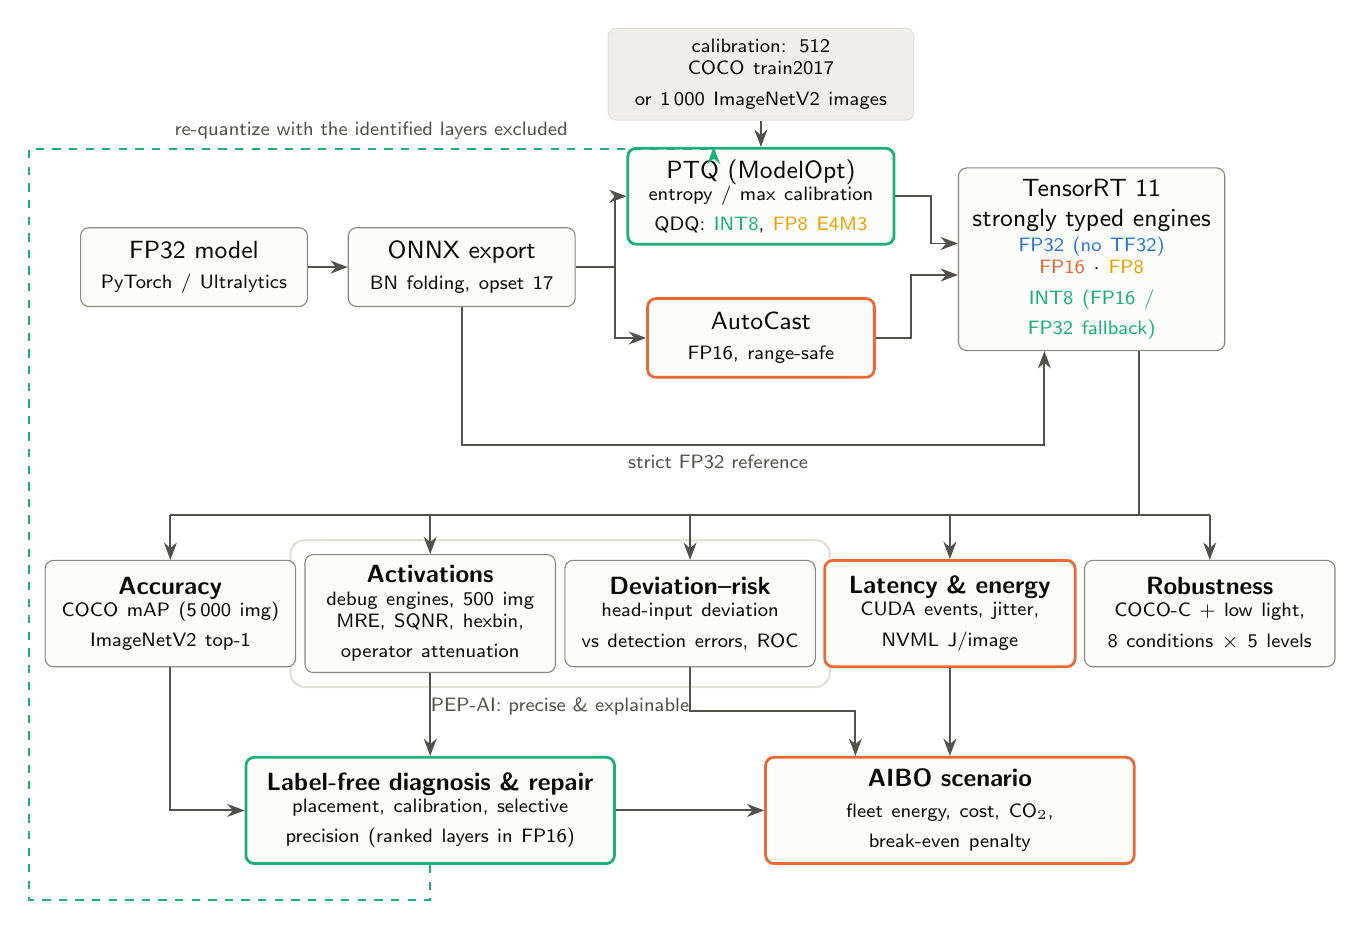
\begin{tikzpicture}
% --- row 1: model preparation (absolute coordinates, cm)
\node[stage] (fp32) at (0,0) {FP32 model\\\scriptsize PyTorch / Ultralytics};
\node[stage] (onnx) at (3.4,0) {ONNX export\\\scriptsize BN folding, opset 17};
\node[stage, draw=int8, line width=1pt, text width=3.1cm] (ptq) at (7.2,0.9) {PTQ (ModelOpt)\\\scriptsize entropy / max calibration\\\scriptsize QDQ: \textcolor{int8}{INT8}, \textcolor{fp8}{FP8 E4M3}};
\node[stage, draw=fp16, line width=1pt] (fp16) at (7.2,-0.9) {AutoCast\\\scriptsize FP16, range-safe};
\node[data, text width=3.6cm] (calib) at (7.2,2.45) {\scriptsize calibration: 512 COCO train2017\\ or 1\,000 ImageNetV2 images};
\node[stage, text width=3.1cm, minimum height=1.6cm] (trt) at (11.4,0.1) {TensorRT 11\\strongly typed engines\\[1pt]\scriptsize \textcolor{fp32}{FP32 (no TF32)}\\ \scriptsize\textcolor{fp16}{FP16} $\cdot$ \textcolor{fp8}{FP8}\\ \scriptsize\textcolor{int8}{INT8 (FP16 / FP32 fallback)}};
\draw[arrow] (fp32) -- (onnx);
\draw[arrow] (onnx.east) -- ++(0.5,0) |- (ptq.west);
\draw[arrow] (onnx.east) -- ++(0.5,0) |- (fp16.west);
\draw[arrow] (calib) -- (ptq);
\draw[arrow] (ptq.east) -- ++(0.45,0) |- ([yshift=2mm]trt.west);
\draw[arrow] (fp16.east) -- ++(0.45,0) |- ([yshift=-2mm]trt.west);
\draw[arrow] (onnx.south) -- ++(0,-1.75) -| node[tag, pos=0.22, below] {strict FP32 reference} ([xshift=-6mm]trt.south);
% --- row 2: measurements
\def\ry{-4.4}
\node[result] (acc) at (-0.3,\ry) {\textbf{Accuracy}\\\scriptsize COCO mAP (5\,000 img)\\\scriptsize ImageNetV2 top-1};
\node[result] (act) at (3.0,\ry) {\textbf{Activations}\\\scriptsize debug engines, 500 img\\\scriptsize MRE, SQNR, hexbin,\\\scriptsize operator attenuation};
\node[result] (risk) at (6.3,\ry) {\textbf{Deviation--risk}\\\scriptsize head-input deviation\\\scriptsize vs detection errors, ROC};
\node[result, draw=fp16, line width=1pt] (energy) at (9.6,\ry) {\textbf{Latency \& energy}\\\scriptsize CUDA events, jitter,\\\scriptsize NVML J/image};
\node[result] (robust) at (12.9,\ry) {\textbf{Robustness}\\\scriptsize COCO-C + low light,\\\scriptsize 8 conditions $\times$ 5 levels};
\coordinate (bus) at (0,-3.15);
\draw[draw=ink2, line width=0.7pt] ([xshift=6mm]trt.south) -- ([xshift=6mm]trt.south |- bus);
\draw[draw=ink2, line width=0.7pt] (acc.north |- bus) -- (robust.north |- bus);
\foreach \n in {acc, act, risk, energy, robust} {\draw[arrow] (\n.north |- bus) -- (\n.north);}
% --- row 3: decisions
\node[result, draw=int8, line width=1pt, text width=4.4cm] (sel) at (3.0,-6.9) {\textbf{Label-free diagnosis \& repair}\\\scriptsize placement, calibration, selective\\\scriptsize precision (ranked layers in FP16)};
\node[result, draw=fp16, line width=1pt, text width=4.4cm] (aibo) at (9.6,-6.9) {\textbf{AIBO scenario}\\\scriptsize fleet energy, cost, CO$_2$, break-even penalty};
\draw[arrow] (act) -- (sel);
\draw[arrow] (energy) -- (aibo);
\draw[arrow] (risk.south) -- ++(0,-0.55) -| ([xshift=-12mm]aibo.north);
\draw[arrow] (acc.south) |- (sel.west);
\draw[arrow] (sel.east) -- (aibo.west);
% --- feedback loop along the left margin
\draw[feedback] (sel.south) -- ++(0,-0.45) -| (-2.1,1.5) -| node[tag, pos=0.25, above] {re-quantize with the identified layers excluded} ([xshift=-6mm]ptq.north);
\begin{scope}[on background layer]
\node[group, fit=(act) (risk), inner sep=5pt, label={[tag, anchor=north]south:PEP-AI: precise \& explainable}] {};
\end{scope}
\end{tikzpicture}
\end{document}
